\newpage
\section{Verification of Lossy Channel Systems}
\label{model}
The goal of this chapter is to formalize the use of \e{small models} for the verification of lossy channel systems, as is done in \cite{parosh}. The technique is based on the use of \e{abstract interpretation} techniques, first formalized by Cousot and Cousot\cite{cousot1977}. Abstract interpretation techniques are techniques of approximating programs. Using information about the control and data flow, i.e. the semantics of a system, an overapproximation of the possible configurations of a system can be created, which is typically an infinite set of configurations. In \cite{parosh} the authors show that such an infinite set of configurations can be safely bounded to a finite set of configurations, by finding a \e{cut-off} point for the maximum size of the evaluations.


\subsection{Views}
\label{subwords}
We define the \e{views} of a configurations \e{c} = $\conf{s,W}$ to be the set $V$ = \{$\conf{s, W'} | W' \subword W$. We say that $views(c) = V$. By definition, the views of a configuration are themselves configurations.

\todo[inline]{Example will be updated.}
\paragraph{Example.} Suppose \e{c} is a configuration $\conf{s_1,s_2,ab,cd}$. The configuration is of size 2 and its views are

\begin{ttabular}
$\conf{s_1,s_2,ab,cd}$ \\
$\conf{s_1,s_2,a,cd}$ &
$\conf{s_1,s_2,b,cd}$ &
$\conf{s_1,s_2,\epsilon,cd}$ \\
$\conf{s_1,s_2,a,c}$ &
$\conf{s_1,s_2,b,c}$ &
$\conf{s_1,s_2,\epsilon,c}$ \\
$\conf{s_1,s_2,a,d}$ &
$\conf{s_1,s_2,b,d}$ &
$\conf{s_1,s_2,\epsilon,d}$ \\
$\conf{s_1,s_2,\epsilon,\epsilon}$ \\
\end{ttabular}


\subsection{Abstraction function}
\label{alphagamma}
For a given parameter $k \in \mathbb{N}$, we use $C$ and $V$ to denote sets of configurations and views respectively, and $C_k$ and $V_k$ to denote configurations and views of size up to $k$.

The abstraction function $\alpha_k: C\rightarrow 2^{C_k}$ maps a configuration $c$ into the powerset $V$ of views of size up to $k$, such that for each $v\in V$, $\{v_eval \subseteq c_eval\}$, $v_state = c_state$ and $size(v_eval) \leq k$ .

\subsection{Concretisation function}
The concretisation function $\gamma_k: 2^{C_k} \rightarrow 2^C$ returns, given a set of views \e{V}, the set of configurations that can be reconstructed from the views in $V$, in other words, $\gamma_k(V) = \{c \in C$ | $\alpha_k(c) \subseteq V$\}

In general $\gamma_k(V)$ is an infinite set of configurations. We define $\gamma_k^l(V)$ := $\gamma_k(V) \cap C_l$ for some $l\geq 0$. The intuitive meaning is that $\gamma_k^l(V)$ is the set of configurations of size at most $l$ for which all views of length at most $k$ are in $V$.

\subsection{Post-Image}
For a configuration $c\in C$ of a lossy transition system $LTS = (C,->)$, we define the \e{post-image} of \e{c} denoted $\rho(c)$ = \{$c'$ | $c \rightarrow c' \in \rightarrow$\}. Intuitively, the post-image of a configuration is the configuration obtained by firing the transitions of the transition system.

For a \e{set} of configurations $V$ we define the post-image of the set $\rho(V)$ = \{$c' | c \rightarrow c' \in \rightarrow, c\in C$\}. This means that the post-image of a set $V$ of configurations is the set $\rho(V)$ containing the post-images of each configurations $c\in V$.

\subsection{Abstract Post-Image}
The \e{abstract post-image} of a set \e{V} $\subseteq$ $C_k$ is defined as $Apost_k$(\e{V}) = $\alpha_k(\rho(\gamma_k(V)))$. This means that the abstract post-image of a set $V$ is the set obtained by applying $\gamma_k$, $\rho$ and $\alpha_k$ in order to the set $V$. The procedure is illustrated in figure \ref{apost}.
\begin{figure}
\abstraction
\caption{The application order of the $\alpha$, $\rho$ and $\gamma$}
\label{apost}
\end{figure}
\todo[inline]{Note to self: When do we say views, when do we say configurations?}

Note that since $V \subset Apost_k(V)$, $Apost_k$ is a monotonic function, and that the set $V$ is a powerset because the function $\alpha$ returns a powerset. This means that by the Tarski fixed point theorem, the function $Apost_k$ has a fixed point.
\todo[inline]{Even the infinte powerset must reach a fixpoint, right?}

\subsection{Reachability Analysis}
\todo[inline]{$\mathbb{R}_k$ was defined in the last chapter, here I would add a section on how to compute it using forward reachability}.


\subsection{Small Models}
\label{proof}
Calculating the abstract post-image of a set of views $V \subseteq C_k$ is essentiatial for the verification procedure. As $\gamma_k(V)$ typically is infinite, this cannot be done straightforwardly. It is the main result of \ref{parosh} that it suffices to consider configurations of $\gamma_k(V)$ of sizes up to $k+1$ ($\gamma_k^{k+1}$), which is a finite set of configurations for which the abstract post-image can be computed. Formally, they show that

\begin{lemma}
\label{lemma1}
For any $k\in\mathbb{N}$, and $X\subseteq C_k$, $\alpha_k(\rho(\gamma_k(X)))$ $\cup$ $X$ = $\alpha_k(\rho(\gamma_k^{k+1}(X)))$ $\cup$ $X$.
\end{lemma}
%\todo{Why is this correct? Shouldn't it be the fixpoint of the two that is equal?}

Below, we show that this lemma holds in the context of lossy channel systems. We show that for any configuration \e{c} $\in$ $\gamma_k(X)$ of size $m > k + 1$ such that there is a configuration \e{c'} where $c' \xrightarrow{r} c$, then for each \e{v'} $\in$ $\alpha_k(c')$, the following holds: There is a configuration \e{d} $\in$ $\gamma_k(V)$ of size at most \e{k}+1 with a transition \e{d} $\xrightarrow{r}$ \e{d'} with \e{v'} $\in$ $\alpha_k(d')$.

\subsubsection{Proofs}
\todo[inline]{The proofs need to be updated, but I await your comments on the definitions in the last chapter. Also, they need a restructuring anyway. Maybe move this to an appendix?}

\paragraph{Transmission rules}
\label{proofTransmission}
%First we note, that for any configuration \e{c} $\in$ \e{V}, any view \e{v'} $\in$ $\alpha_k(c)$ is also a valid configuration \e{v'} $\in$ $\gamma_k(V)$, since $\alpha_k(v')$ $\subseteq$ $\alpha_k(c)$ and thus \e{v'} $\in$ $\gamma_k^{k+1}(\alpha_k(c))$. Also note that if from \e{c} a transition \e{r} can be fired, then this transition can also be fired from any configuration \e{c'} = \e{v'}, as transmission rules are guarded only by the states of the channel system and not by channel evaluations.

%A transmission rule changes the evaluation of at most one channel \e{ch} $\in$ \e{c}, and (possibly) the state of the channel system, thus we need only reason about the evaluations of a single channel \e{ch}.

%Let \e{c} = $\conf{S, w}$ $\xrightarrow{ch!w_{m+1}}$ $\conf{S', w \bullet m}$ = \e{c'}.

%The views of \e{c'} of size up to k are either of the type 1) $\conf{S', w' \sqsubset w}$, with size($w'$) $\leq$ $k$ (i.e. not including the newly transmitted message) or 2) of the form $\conf{S', w' \bullet m | w' \sqsubseteq w}$ with size($w'$) < $k$.

%For any view of type 1, there exists a configuration of size $k$, \e{d} = $\conf{S, w'}$ $\in$ $\alpha_k{c}$ and the transition $r$ can be taken, resulting in \e{d'} = $\conf{S, w'\bullet m}$ of size $k$+1. The view \e{v'} $\in$ $\alpha_k{w'}$.

%For any view of type 2, there exists a configuration of size $k-1$, \e{d} = $\conf{S, w'}$ and the transition $r$ can be taken resulting in \e{d'} = $\conf{S, w'\bullet m}$ = $v'$.

%\e{Example}. Assume a system with two processes and a single channel. Let \e{c} = $\conf{1,2,abc}$ $\rightarrow{ch!d}$ $\conf{2,2,abcd}$. Assume that $\e{c}$ $\in$ $\gamma_2(V)$, then $\alpha_2(c)$ $\in$ \e{V}, i.e. $\conf{1,2,a}$, $\conf{1,2,b}$, $\conf{1,2,c}$, $\conf{1,2,ab}$, $\conf{1,2,bc}$, $\conf{1,2,ac}$ are in in V and also in $\gamma_k(V)$.

%$\alpha_2(c')$ = \{$\conf{2,2,a}$, $\conf{2,2,b}$, $\conf{2,2,c}$, $\conf{2,2,d}$, $\conf{2,2,ab}$, $\conf{2,2,bc}$, $\conf{2,2,cd}$, $\conf{2,2,ac}$, $\conf{2,2,ad}$, $\conf{2,2,bd} $ \}. Consider a view with the newly transmitted message, $\conf{2,2,cd}$, it can by created by $\conf{1,2,c}$ $\rightarrow{ch!d}$ $\conf{2,2,cd}$. Considering instead a view without the transmitted message, $\conf{1,2,ab}$, it can be created by $\conf{1,2,ab}$ $\rightarrow$ $\conf{2,2,abd}$ for which $\conf{2,2,ab}$ is a view.

\paragraph{Reception rules}
\label{proofreception}
%As opposed to the transmission rules, reception rules rely both on the state and the evaluation in order to be fired, but only the state of a single channel need be considered.

%Consider a configration \e{c} = $\conf{S, m\bullet w}$ $\xrightarrow{ch?m}$ $\conf{S, w}$ = c', such that $size(c)$ $\geq$ $k+1$. For any view \e{v'} $\in$ $\alpha_k(c)$ with the word \e{w'} of size at most \e{k} on the channel, there exists a configuration $d$ of size at most \e{k+1}, \e{d} = $\conf{S, m\bullet w'}$ $\in$ $\alpha_k(c)$ such that \e{d} $\xrightarrow{ch?m}$ \e{d'} = \e{v'}.

\paragraph{Actions}
%Actions can in this context be seen as equivalent to a reception rule, reading the empty symbol $\epsilon$ on some channel. The proof then follows directly from \ref{proofreception}.
\subsection{Verification Algorithm}
\label{implementation}
As a result of lemma \ref{lemma1}, if $\gamma_k^{k+1} \cap Bad$ = $\empty$ for any \e{k} $\geq$ 1, then $\gamma_k(V) \cap Bad$ = $\empty$ for any larger \e{k}. Given a set of bad states \e{Bad}, a set of initial states \e{I} and a set of transitions, Verification of a system can be done with algorithm \ref{alg1}, which was first presented in \cite{parosh}.

\begin{algorithm}
  \caption{General Verification algorithm}
  \label{alg1}
    \hspace{8pt}\textbf{for} $k := 1$ \textbf{to} $\infty$

    \hspace{16pt}\textbf{if} $\mathcal{R}_k$ $\cap$ $Bad$ $\neq$ $\emptyset$ \textbf{then return} Unsafe

    \hspace{16pt}$V := \mu X.\alpha_k(I)$ $\cup$ $Apost_k(X)$

    \hspace{16pt}\textbf{if} {$\gamma_k(V)$ $\cap$ $Bad$ = $\emptyset$} \textbf{then return} Safe
\end{algorithm}

The algorithm begins by performing a reachability analysis in order to compute $\mathcal{R}_k$ and check for bad states. For any buffer size \e{k}, if a bad state is found to be reachable in $\mathcal{R}_k$, the system is unsafe and the algorithm terminates. If no such bad state was found, the algorithm continues by computing an \e{overapproximation} of configurations of size $k$, reachable through configurations of size at most $k+1$ and checking for bad configurations. This is done by computing $Apost_k$ iteratively until a fixpoint \e{V} is reached. If at this point no bad configuration has been found, the system can be said to be safe (due to the result of \ref{lemma1}) and the algorithm terminates. If on the other hand a bad state was found, the system is not necessarily unsafe, as \e{V} is an over-approximation of the reachable states in $\mathcal{R}_k$, the process is repeated with a buffer size of \e{k+1}. This process is abstractly described in the flowchart in figure \ref{flow}.

\begin{figure}
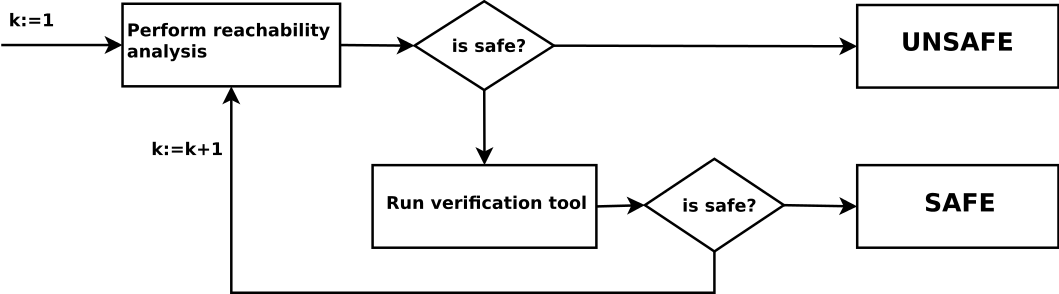
\includegraphics[width=400pt] {bilder/flowchart.png}
\caption{The general flow of the verifier.}
\label{flow}
\end{figure}
